\chapter{GPU Programming}
\label{chap:gpu}

Moore's law has driven the rise of processor performance for a long time -- \enquote{The complexity for minimum component costs has increased at a rate of roughly a factor of two per year. Certainly over the short term this rate can be expected to continue, if not to increase. Over the longer term, the rate of increase is a bit more uncertain, although there is no reason to believe it will not remain constant for at least 10 years} \citep{MooresLaw}. This \enquote{law}, if we may call it that way, is unfortunately limited by the physical properties of components used within modern processors. 
These boundaries are both on the side of transistors size and their quantity in the processor core, as well as on the side of maximum processing speed. 
Over the last years, scientists are predicting the end of Moore's law \citep{MooresLawEnd}, and their voices are more turbulent since the size of transistors in the \acrfull{acc:cpu} reached $7nm$ in 2018 \citep{SamsungSevenNm}. 

Processor manufacturers are well aware of the physical complications stemming from the transistors' small size and invest more effort into multi--core processors. These processors have many independent cores that can be utilized in parallel, and can possibly increase the processor's performance linearly with respect to the number of cores. To name a few, last Intel's server processors Xeon\textsuperscript{\textregistered} Platinum 8380 Processor with 40 cores and 80 threads \citep{IntelXeonPlatinum}, as well as AMD's EPYC\texttrademark\ 7763 with 64 cores and 128 threads, are great examples \citep{AMDEpyc}.

\acrfullpl{acc:gpu}\index{GPU} takes this idea of multi--core processors further. Rather than increasing single--thread performance, the \gpu manufacturers are focusing on massive parallelism using a vast number of cores operating in highly parallel and distributed manner \citep{GPUComputingOwens}. Using this strategy, the \gpu programming offers encouraging performance for heavy workloads. Common consumer \acrshortpl{acc:gpu} can easily outperform current high--end \acrshortpl{acc:cpu} in the instruction throughput and memory bandwidth. These demands came originally from the game industry, which places great emphasis on parallel processing and reasonably real--time latency.

The decisions regarding the architecture, though, affect the way \acrshortpl{acc:gpu} are programmed. Unlike a \cpuns, which can run generic code, a \gpu is more suited for specific classes of algorithms that can fully utilize the underlying hardware. Engineers recognized the following mandatory properties of the efficient application running on \gpu \citep{GPUComputingOwens}:
\begin{itemize}
    \item \textit{Large computation demands} -- \gpu can deliver tremendous performance but may be slow for short tasks without sufficient data. The overhead of memory allocation on \gpu and moving it forth and back to \cpu can quickly outweigh the advantage of using it. On contrary, the real--time rendering requires hundreds of operations per pixel, and \gpu can easily meet these demands. \gpu is furthermore hiding memory access latency behind more computations (I will talk about it a bit later); it needs therefore sufficient amount of work to do that.
    \item \textit{Significant parallelism} -- the algorithm needs to parallelize easily and ideally scale to as many cores as possible. Whereas \cpu provides tens of cores (up to 64 today), the \gpu has hundreds or thousands of them (current cutting-edge \gpu produced especially for \acrshort{acc:ai}, NVIDIA V100, has 5120 CUDA cores \citep{nvidiav100spec}), although with limited per--core performance. If an algorithm can employ only a few of them, it may be slower than on multi--core \cpu. Once again, real--time rendering can render each pixel independently, making it a perfect candidate for \gpu computing.
    \item \textit{Throughput over latency} -- because the \gpu is highly parallel by design, the throughput is more important than the absolute latency of individual operations. From the point of rendering, the human eye can perceive images in order of milliseconds. Operations in modern processors take in the order of nanoseconds. Therefore, the absolute time to render a single pixel is not relevant as long as the whole picture is rendered bellow noticeable time. The algorithms cannot make assumptions about the running time of individual parts but rather on the task running time as a whole.
\end{itemize}

\acrlong{acc:ea} fits well into these categories, as the algorithm may evaluate individuals' fitness in parallel, and the evaluation is independent in respect to the rest of the population. The crossover and mutation operators may be easily parallelized as well, as they operate on individuals (or a small set of individuals) independently. We may parallelize the algorithm even more by processing each gene separately, as presented by \citet{CHENG2019514}. I will discuss this option at the end of this chapter.




%%%%%%%%%%%%%%%
%%           %%
%%  HISTORY  %%
%%           %%
%%%%%%%%%%%%%%%
\section{History}

Historically, \gpu came from the demand of the game industry for real--time rendering. In the rendering process, a list of geometric primitives, usually triangles, is processed through a number of stages to produce a final picture. The primitives can be processed independently and therefore in parallel, which makes real--time rendering the ideal case for the application of \gpuns. The typical operations in graphical pipeline consists of \citep{GPUComputingOwens}\index{rendering pipeline}:
\begin{itemize}
    \item Vertex stage that transforms and calculates properties per vertex. Typical operations are transforming vertex position from world space (that is, the coordinates in the scene) into screen space (that is, the coordinates in respect to the viewer point of view) and estimating further vertex properties like color, material, or texture coordinates.
    \item Primitive assembly transforms geometric primitives into triangles -- the standard geometric primitive for \gpu to work with. This stage may also clip the primitives that are not in the observer's view and save some computation in the following stages.
    \item Rasterization takes generated triangles and resolves which pixels correspond to the provided triangle. These pixels do not necessarily need to match the number of pixels of the screen. They are usually referred to as fragments -- for example, the superscaling technique renders the scene in higher resolution and then downsample it to match screen resolution \citep{GameGraphicProgramming}. Each triangle may be composed of hundreds or thousands of fragments. Moreover, the rasterization typically interpolates vertex properties between the fragments.
    \item Fragment stage processes each fragment and typically resolves the final appearance of the fragment. It may calculate fragment interactions with the lights in the scene, fetch colors from textures, blend fragments, etc. This stage is usually most demanding, as a typical scene consists of millions of fragments.
    \item Composition stage assembles all the fragments into a final image. It may, among others, test fragments visibility, depth, and do stencil filtering.
\end{itemize}

The stages \gpu performs are usually referred to as \emph{rendering pipeline} and may have slight variations on different hardware. In the beginning, the stages discussed earlier have been preprogrammed by the manufacturer, and developers had only limited options of how to control the pipeline stages (also known as the fixed--function pipeline). As the software complexity increased, the need for more control arise, and the manufactures provided a way to program the individual stages of the pipeline. These programs are called \emph{shaders} and their capabilities matured over the years. In 2006, Microsoft introduced Shading Model 4.0, which allowed using the same programming interface and hardware both for vertex and fragment shader \citep{DirectX10}. Not only that, but more stages appeared (like tessellation and geometry shaders) to provide developers more control over the pipeline. Today, two major \acrfull{acc:api} exists -- proprietary  DirectX and open--source OpenGL. Note that some stages of the rendering pipeline, such as primitive assembly, rasterization, and composition, are still implemented by the \gpu manufacturers and, in most cases, are implemented by special--purpose hardware components (because of the performance reasons) \citep{SoftwareRasterization}. They are, hence, integral components of the rendering pipeline and are not possible to modify.

Soon, scientists and engineers recognized many more problems that would benefit by \gpu performance. Although some stages of the rendering pipeline were fully programmable, the pipeline was still inherently graphical, and some stages were not possible to skip. Executing general--purpose programs on \gpu required encoding the problem in the domain of geometric primitives and use available programmable and special--purpose hardware to implement the algorithm. Moreover, the programmers need to decide which part of the hardware will execute which part of the calculation and how the pipeline's fixed stages will affect the data structure. As shader programs do not have access to shared memory, the data passing was realized using textures, vertices, and fragment properties \citep{GPUComputingOwens}. These difficulties discouraged wider adaption of \gpu for general--purpose programs, although some efforts have been made to hide the underlying rendering pipeline from the programmer point of view \citep{BrookGPU}.

Lack of support for general--purpose program on \gpu inspired companies to develop a new approach that would provide programmers better control over the underlying hardware. In 2006, NVIDIA introduced first version of \acrfull{acc:cuda}\index{CUDA} \citep{CUDAabout}. Open--source standard of general--purpose \gpu programming came in 2008 as Open Computing Language (OpenCL) by Khronos Group \citep{OpenCLRelease}. These are higher--level interfaces with C--like syntax exposing \gpu resources without any connection to the graphical pipeline. Programmer is given control of execution and parallelization of the program, as well as memory access. Over the years, these technologies undergo various improvements (the current version is CUDA 11.2, respectively OpenCL 3.0), adding support for data types, language constructs, and new hardware.

\cuda become de facto standard in the field of general--purpose computing on \gpu and I will focus mainly on it. Fortunately, other technologies like OpenCL have similar underlying architecture and approach to the \gpu programming. The following section should hence generalize for them as well.




%%%%%%%%%%%%%%%%%%%%
%%                %%
%%  ARCHITECTURE  %%
%%                %%
%%%%%%%%%%%%%%%%%%%%
\section{Architecture}

The design goal of \gpu is to provide orders of magnitude higher instruction throughput and memory bandwidth compared to \cpuns. The overall architecture of \gpu is therefore significantly different. This section will focus on \gpu architecture from the point of \cuda platform, taking inspiration mainly from the CUDA Programming Guide \citep{CUDAguide}.

\begin{figure}
    \begin{subfigure}[t]{0.47\textwidth}
        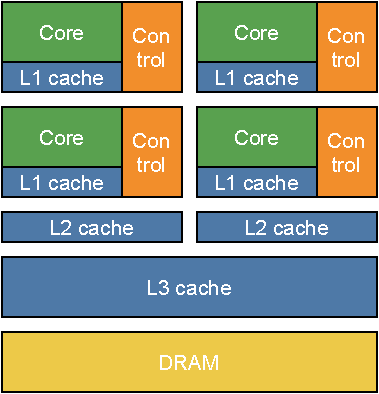
\includegraphics[width=\textwidth]{img/master_cpu_arch.pdf}
        \caption{Architecture of \acrshort*{acc:cpu}. Each core has L1 cache and own control circuit. Cores can therefore work independently.}
        \label{fig:cpuarch}
    \end{subfigure}
    \hfill
    \begin{subfigure}[t]{0.47\textwidth}
        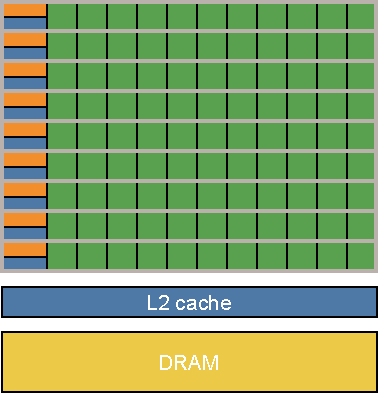
\includegraphics[width=\textwidth]{img/master_gpu_arch.pdf}
        \caption{Architecture of \acrshort*{acc:gpu}. One control circuit controls number of cores. One row of cores is called \acrlong{acc:sm} (\acrshort{acc:sm}, bounded by gray borders). L2 cache is shared between the cores.}
        \label{fig:gpuarch}
    \end{subfigure}
    \caption{Difference between \acrshort*{acc:cpu} and \acrshort*{acc:gpu} architecture}
\end{figure}

The computation power of \gpu emanates from the point that it dedicates more transistors on the chip to the data processing rather than to the control circuitry. The architecture of the \cpu is shown in Figure \ref{fig:cpuarch}. Each core has its own control circuit, and therefore each core can execute instructions independently. Moreover, each thread has its own L1 cache.

The \gpu\index{GPU architecture} architecture is portrayed in Figure \ref{fig:gpuarch}. A set of cores share the same control circuitry and L1 cache. One line of these cores is called \acrfull{acc:sm}. The exact number of cores per \acrshort{acc:sm} differ between architectures; more information can be found in the article by \citet{NVIDIAhistory} or on NVIDIA official websites. Using one control circuitry to manage many cores brings some implications -- all the cores need to administer the same instruction at once. In this sense, the instruction throughput is achieved using \acrfull{acc:simd} approach -- one instruction can at one tick alter multiple data on multiple cores.

Each \gpu comes with a different set of hardware and software features. Compute capability\index{CUDA!compute capability} specify which features are available on the target system. For example half--precision float--point operations are available since compute capability 5.3. The number of arithmetic CUDA cores per \acrshort{acc:sm} is 8 for compute capability 1.x, 32 resp. 48 for compute capability 2.0 resp. 2.1, 64 for compute capability 6.0, 7.x, and 8.0, 128 for compute capability 6.1, 6.2, and 8.6, and finally 192 for compute capability 3.x. I will not discuss specific compute capability in the following text. I will assume compute capability of at least 6.0 through this work, but I do not depend on the concrete version, as they should be backward compatible. In order to use newer compute capabilities, the \gpu, driver, and the software need to support them.

\acrlong{acc:cuda} allows almost direct translation of code from C onto the \gpuns. It uses \cpp language with a few extensions. It is therefore straightforward to write a program for \gpuns, as long as we are familiar with C syntax. To distinguish code running on \cpu and \gpu, \cuda differentiate between host (the code running on \cpu) and device (the code running on the \gpu) functions. There is a particular type of function called \emph{kernels}\index{CUDA!kernel}, which is evoked by the host but executed on the device.

The \cuda defines the following terminology:
\begin{itemize}
    \item CUDA thread\index{CUDA!thread} is execution of a single kernel. To process $K$ blocks of data, the runtime creates at least $K$ threads and runs the same kernel function on each of them.
    \item CUDA thread block\index{CUDA!block} is a collection of threads grouped into the grid. The programmer may specify the size of the grid during the call of the kernel function as a three-dimensional vector. The maximum number of threads in the thread block is limited by the compute capability of the hardware. Moreover, all the threads in the thread block need to be executed on one \acrshort{acc:sm} (with some exceptions) and can be synchronized using \textit{\_\_syncthreads} call. Each kernel receives \textit{threadIdx} variable, which allows identifying individual threads in the block.
    \item CUDA kernel grid\index{CUDA!grid} is a grid of thread blocks. Similarly to thread block, its size may be specified during kernel invocation, and each thread receives \textit{blockIdx} resp. \textit{blockDim} variables identifying block in which the thread is running, resp. size of the blocks. More blocks from the same grid may run in parallel on different or same \acrshort{acc:sm} (if the \acrshort{acc:sm} have free capacity), but the threads from distinct blocks cannot be synchronized.
    \item Warp\index{CUDA!warp} is a set of 32 threads (for all compute capabilities so far) that execute the same instruction. The thread block is split into warps and executed by the \acrshort{acc:sm}. The warp is the minimal unit executable on the \gpu. The device plan warps the same way \acrshort{acc:os} plans processes and may switch context to another warp while the current one is waiting for the data. By executing different warp, the latency of, for example, memory access is \enquote{hidden} behind the execution of different warp -- known as hiding latency behind computation. Although \gpu cannot execute anything smaller than the warp (like a single core), it may mask some threads from the execution. Therefore, it is possible to have a block size of $50$ threads; however, $2\cdot32 - 50=14$ cores in the second warp will still execute the kernel without any effect (this matter is hidden from the programmer).
\end{itemize}

Because \cuda assumes a system composed of host and device, each of them has its own separate memory. The kernel is executing on the device and, as such, needs to have data its operating on moved into the device memory. \cuda provides a set of functions to allocate, deallocate, copy, and move memory between the host and the device\index{CUDA!memory management}. Similar to traditional \cpp programming, \cuda memory is allocated in a single unified linear address space. It can reference other addresses using pointers and use advanced data structures like linked lists and trees. Yet, the data movement between host and device is time--consuming, because the bandwidth between \cpu and \gpu is lower than memory transfers within the device memory. The copy of memory from the host to the device may generate nontrivial overhead that may waive the advantage of using \gpu altogether, especially for small kernels. 

To reduce access latency to global device memory, \cuda provides a set of tools to speed up the process. It is possible to control the L2 cache policy to better match workloads of executing kernels. It also provides functions to manage \emph{page--locked host memory}, which remains in the host memory and will not page by the \acrshort{acc:os}. Copying from this kind of memory can be done asynchronously, or when allocated as \emph{mapped--memory}, it is shared between the host and the device. Mapped--memory is implicitly transferred to and from the device, and the programmer does not need to allocate it explicitly.

A special kind of memory, residing on--chip, is \emph{shared memory}\index{CUDA!shared memory}. The latency of shared memory is roughly 100x times lower than for global device memory, and the memory is shared in the thread block. Simple operations like matrix multiplication can hasten by order of magnitude using shared memory \citep{MatrixMultiplicationGPU}. However, shared memory operates in equally--sized memory modules called banks, which complicates concurrent access to the shared memory. All the compute capabilities up today have 32 banks for shared memory organized into 32--bit words. Access to distinct memory addresses belonging to the same bank (bank conflict) by multiple threads within the same warp is serialized and, therefore, significantly increases the kernel's running time. This is common for data types with 64--bits, such as double--precision floats. It may be beneficial to pad each value with one byte to eliminate conflicting access to the same banks.

As I mentioned earlier, all threads in the warp need to execute the exact same instruction. However, the programming language supports conditional jumps, loops, and other constructs known from the modern programming languages. It may certainly happen that some threads within the warp may execute different execution path -- a situation known as \emph{warp divergence}\index{CUDA!warp divergence}. There are further causes, why the threads in the warp may diverge, but the branching is the most common one. In order for \gpu to evaluate each execution path, it executes the branched paths sequentially and masks out threads not participating in the current one. Masked threads will execute the program; however, their results are ignored from the programmer point of view. This implies the same code will be executed twice (note that this grows exponentially for nested conditions) and significantly extend the time to finish the program. In general, warp divergence is undesirable and should be avoided when possible.
Warm divergence can only occur within a warp. Different warps in the same thread block may execute different execution paths without any impact on the program's performance.

The parallel nature of \cuda helps several algorithms that have by order of magnitudes better performance on \gpu than on \cpuns. A typical example would be element--wise linear operations or matrix multiplication \citep{GPUMatrixMultiplication}. Reduction operations such as summation of the array can be implemented effectively on \gpu \citep{harris2007optimizing}, as well as different kinds of sorting algorithms \citep{GPUsorting}.

These operations are so popular, NVIDIA released a set of libraries with the implementation of these algorithms. The most relevant for this work are \textit{cuBLAS} (\gpuns--accelerated basic linear algebra library), CUDA Math Library implementing most common mathematical functions, and \textit{cuRAND} (\cpuns--accelerated random number generation). These implementations are optimized for the latest hardware and maintained by NVIDIA.




%%%%%%%%%%%%%%%
%%           %%
%%  PYTORCH  %%
%%           %%
%%%%%%%%%%%%%%%
\section{PyTorch}

From the brief description of \cuda above is clear that programming in \cuda is fundamentally different from programming in traditional programming languages like C or \cppns. The efficient implementation of kernels is complex, and in order to fully use the power of \gpuns, the programmer needs to understand the underlying hardware. Not an ability commonly found among scientists and engineers dealing with evolutionary algorithms. As one of the goals of this thesis is to provide easy--to\kern0.1em--use and extend library for evolutionary algorithms, I decide to look for an alternative.

PyTorch\index{PyTorch} is free open--source library maintained by Facebook's AI Research lab (\href{https://ai.facebook.com/}{FAIR}). It builds on top of \href{http://torch.ch/}{Torch} library for scientific computing on \gpuns. It is possible to use \cpp or Python programming languages to implement applications using PyTorch library, where the Python language is the primary language the library focuses on. I argue that more programmers are familiar with Python language than with C or \cppns; and its use is hence more plausible than \cuda for my purpose \citep{StackOverflowSurvey}. PyTorch hides the underlying kernels behind a unified interface, and the programmer does not need to know \cuda programming at all. When necessary, PyTorch allows implementing parts of the algorithm in \cpp or even as a native \cuda kernel and chain it with the rest of the PyTorch library \citep{PyTorchDoc}. The end--user may call this native implementation directly from Python source code without noticing it. This approach allows optimizing specific parts of the algorithm if the performance is not pleasing.

The building block of PyTorch library is the \incode{torch.Tensor} data type\index{PyTorch!data types}. It represents a multidimensional array of scalars. PyTorch allows to define the type of the scalars to be the same as supported by most of the programming languages, the most common are 16, 32, or 64--bit floating--points numbers (also known as half--precision, single--precision, and double--precision floating--point formats), signed 8, 16, 32, and 64--bit integer numbers (also known as char, short, integer and long numbers), 8--bit unsigned integer (known as byte), and Boolean data type storing either 1 (true) or 0 (false) values. Except for these, PyTorch supports 32, 64, and 128--bit complex numbers.

Tensors are efficiently stored in memory by setting the size and stride of each dimension. This allows representing $k$-dimensional tensor of constant value by only a single value in memory. We set the desired size of each dimension and stride equal to $0$. Because PyTorch kernels anticipate tensors in this format (with size and stride defined), they will automatically reference the single value instead of duplicating it in the memory. There is also the possibility to store sparse tensors using the \incode{torch.sparse} package and keep in memory only non--zero values. Note that sparse tensors are only in beta \citep{PyTorchDoc}.

The kernels are realized as operations with tensors\index{PyTorch!operations}. PyTorch provides a broad range of operations, highly similar to the functions in the NumPy library, which is de facto standard for numeric computation algorithms in Python. These functions are also similar to MATLAB numerical functions, and very presumably, programmers coming from other platforms may effectively implement their algorithms in PyTorch because the \acrshort{acc:api} is familiar to them. This is one of the reasons why I choose PyTorch as the library for the implementation of evolutionary algorithms.

PyTorch functions realize standard algebraic operations, geometric and statistical functions, matrix multiplication, bitwise operations, reduction operations like summation, finding unique elements, or logical testing of the list of variables. Moreover, PyTorch implements functions from BLAS (Basic Linear Algebra Subprograms) specification and LAPACK (Linear Algebra Package) library like matrix decomposition, linear equations solver, determinant, and much more \citep{PyTorchDoc}.

For pseudo--random number generation PyTorch uses underlying implementations -- either Mersenne Twister for CPU or Philox implemented in NVIDIA's cuRAND library. The latter is efficient for \cuda programming, but need to be initialized by each thread before the generation. Historically, people were generating random numbers on \cpu and moving them to \gpu afterward. Using native \cuda implementation is without a doubt more effective.

The advantage of PyTorch is that its functions are implemented both for \cpuns, as well as for \gpuns. It is possible to use the same source code without any changes on machines without \gpuns. The implementation may still use \acrshort{acc:simd} instructions on \cpuns, that are ordinarily available on modern processors (also known as vectorized instructions). Note that although these are still \acrshort{acc:simd} instructions, the performance is not nearly as good as running all the computations on \gpu in parallel. Nevertheless, the performance would still be a bit better than using C or \cpp purely without optimization.

Another advantage of using an existing library like PyTorch is that the implementation (and especially the \cuda kernels) is written and maintained by a team of professionals that understand the architecture and working of the \gpu most likely better than most of the people dealing with evolutionary algorithms. Using existing frameworks gives assurance the kernels are implemented efficiently both on the \gpu and \cpuns. What is, in my opinion, more important is that the library is kept up--to--date and may use features of new, not yet released hardware, in the future. All we need to do is to update the library, and the same source code may use the new hardware and features.

Because of the PyTorch properties mentioned above, I decided to implement the evolutionary algorithms in this framework.




%%%%%%%%%%%%%%%%%%%%%%%%%%%
%%                       %%
%%  EVA PARALLELIZATION  %%
%%                       %%
%%%%%%%%%%%%%%%%%%%%%%%%%%%
\section{Evolutionary Algorithms parallelization}

General \acrlong{acc:ea} manage a population of individuals and by repeated application of evolutionary operators search for the optimal solution of the problem at hand. As the individuals within the population are independent, there is excellent potential to speed up the whole process by parallelizing evolutionary operators. Although some of the operators need more than one individual for their execution (the crossover operators are the typical example), the operator is, in most cases, applied several times on different sets of individuals. Further, these sets are usually small, and the operator may be executed in parallel for all of them. The typical crossover operator, for example, needs only two individuals and is applied repeatedly on different parents.

Scientists and engineers were well aware of this potential, and the first attempts \citep{PGAPack} to parallelize evolutionary algorithms came long before \cuda was introduced by NVIDIA in 2006. These projects were either using a single machine with multiple processor cores or a system of machines sharing the population over the network. The common idea is to divide the population into chunks and solve them simultaneously using multiple processors. There are two way of doing that \citep{CHENG2019514}:
\begin{itemize}
    \item Master--worker model executes all the evolutionary operators on a single machine, but the fitness evaluation is spread among several processors. While the fitness evaluation takes a significant amount of time (for example, run of a physical simulation is very time--consuming), and the time to share the individuals among processors is negligible, the master--worker model is the best way to accelerate the algorithm.
    \item Island model maintains a list of populations evolving independently. Each of these populations may run on a separate processor and therefore in parallel. The populations are usually called \emph{islands} because from the evolutionary point of view appear as evolutions on different continents. The islands do not collaborate with each other, except a specific operator called \emph{migration operator}\index{migration operator}. This operator periodically, in a predefined way, exchanges a small portion of the population among the islands. By borrowing few individuals from a different island, we hope to bring new genetic material. It has been shown that the island model on its own may improve the solution quality and running time of the algorithm \citep{IslandModel}.
\end{itemize}
These models are historically more suited for multi--processor systems rather than for \gpuns, as it would be hard to scale them up to thousands of cores currently available in modern \gpuns. Nevertheless, these approaches can still be combined with the proposed implementation. One may, for example, use the island model and run each population on a different \gpuns--enabled machine.

\begin{figure}[hb!]
    \centering
    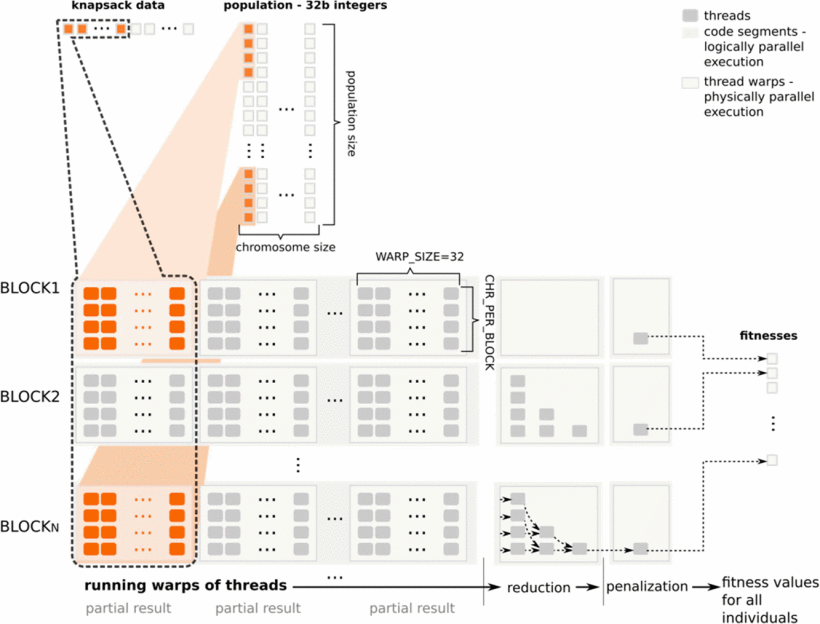
\includegraphics[width=0.7\textwidth]{img/KnapsackKernelDesign.png}
    \caption[Knapsack problem CUDA evaluation kernel]{Design of the knapsack fitness function kernel in \citet{GpuIsland}. It is gene--level model, where each thread aggregate informations from one individual and $CHR\_PER\_BLOCK$ items.}
    \label{fig:knapsackkernel}
\end{figure}

In parallel computing, the granularity\index{granularity} is a measure of the computation amount conducted by the task. Typically, there is coarse--grained parallelism, which splits the problem into several large tasks. Fine--grained parallelism, in contrast, breaks the problem into a large number of small tasks. Both coarse--grained and fine--grained algorithms have been proposed for \cpu architecture. For \gpu programming, however, more delicate levels of granularity are needed:
\begin{itemize}
    \item Chromosome--level granularity evaluate one individual using one thread. Master--worker model mentioned earlier is an example of the chromosome--level granularity. For \cuda purposes, this degree of granularity is still too raw.
    \item Warp--level granularity evaluate one individual using warp of threads. The advantage of warp is that threads within may communicate, and for some problems, this may be necessary to do so.
    \item Gene--level granularity evaluate each gene using one thread, or more generally evaluate one individual using more threads (then warp--level granularity is just a special case of the gene--level granularity).     
\end{itemize}
The gene--level granularity is ideal for the \gpu computing, as it exposes enough parallelism. Earlier attempts with chromosome--level or more coarse level granularity could not fully utilize the \gpuns. One example of the gene--level granularity is in the work of \citet*{GpuIsland} for the knapsack problem. His design of the \cuda kernel is in the Figure \ref{fig:knapsackkernel}. Other authors implemented various algorithms using \cudans, for example, simple genetic algorithm \citep{SimpleGACUDA}, differential evolution \citep{veronese2010differential}, and particle swarm optimization \citep{PSOCUDA}. All of them showed orders of magnitude speedup and proof that implementing \acrlong{acc:ea} on \gpu has its advantages.
